\begin{figure}[t]
\centering
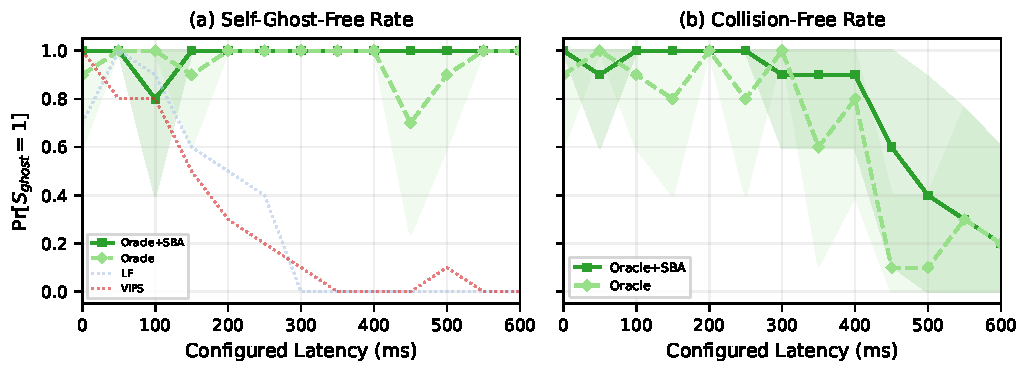
\includegraphics[width=\columnwidth]{figures/oracle_isolation.pdf}
\caption{Oracle baseline. (a) Self-ghost-free rate stays near 1.0 across all latencies, confirming that single-source perception eliminates ego-consistent duplicates by construction. (b) Collision-free rate degrades at high latency due to physics. The gap between the Oracle physics bound and the multi-source logic cliff quantifies the cost of identity ambiguity.}
\label{fig:oracle_isolation}
\end{figure}
